% !TeX spellcheck = es_ES
% !TeX encoding = UTF-8

\section{Explicación del programa}

\definecolor{minimalgrey}{rgb}{0.99, 0.99, 0.99} % Propia invención

\setminted{style=pastie, bgcolor=minimalgrey, breaklines, linenos, tabsize=2}

Cuando se trabaja con grandes cantidades de datos calcular la media a través de métodos convencionales es muy costoso operacionalmente; en estas ocasiones utilizamos una aproximación de la media a través de muestras. Para estar seguros de que la aproximación es relativamente correcta se establecen hipótesis y sus posibilidades de cumplirse se contrastan con un error permitido.

\medskip
Para empezar se cargan los datos de los cuales se desea calcular la media.

\inputminted[firstline=7, lastline=9]{R}{../R/media.R}

Las muestras previamente comentadas se toman en potencias de $2$ usando $k$ como exponente de la operación $2^k$, empezando con $k = 2$, para dejar un número menor a la hipótesis. Para tomar estas muestras se utiliza la función \textit{obtener\_sample} la cual devuelve la media y la varianza de la muestra junto a la muestra.

\inputminted[firstline=2, lastline=7]{R}{../R/dependencias.R}

También hay que conseguir una hipótesis (\textit{contrastar}) inicial, la cual se guarda en una variable, se utiliza $k-1$ para obtener una hipótesis con muestra menor a la muestra a la que se contrasta, encima sabemos que en esa línea $k=2$ con lo que se cogerá una muestra de tamaño 2 (la más pequeña posible):

\inputminted[firstline=14, lastline=14]{R}{../R/media.R}

La primera hipótesis es bastante probable que no se pueda asegurar con la certeza que se desea, con lo que todo el código a partir de este momento deberá estar dentro de un bucle, en este caso se usa un $while$ bajo la condición de que una boolean llamada $CONTINUE$ sea $true$.

\medskip
Para empezar, hay que asegurarse que la muestra que se coge no sea mayor que la cantidad de datos que tenemos, ya que no tiene sentido seleccionar $1500$ datos de una selección de $1000$. Para ello se utiliza este fragmento de código:

\inputminted[autogobble, firstline=19, lastline=23]{R}{../R/media.R}

A continuación se debe decidir si se quiere utilizar una distribución tipo T-Student o una distribución normal, para ello se utiliza la función \textit{distribucion\_correcta} que basándose en la cantidad de datos que tiene nuestra muestra decide la distribución adecuada en cada caso.

\inputminted[firstline=10, lastline=16]{R}{../R/dependencias.R}

Pero aunque el tamaño de la muestra es de gran utilidad, todavía tenemos que calcular la muestra, para ello se reúsa la función \textit{obtener\_sample} previamente mencionada; para guardar los datos los diferentes datos que devuelve, se debe utilizar el siguiente fragmento de código:

\inputminted[autogobble, firstline=28, lastline=31]{R}{../R/media.R}

Una vez obtenida la muestra, obtener la d.t. y la posición opuesta del contrastador es el siguiente paso:

\inputminted[autogobble, firstline=33, lastline=34]{R}{../R/media.R}

\inputminted[firstline=18, lastline=24]{R}{../R/dependencias.R}

Ahora queda la parte más difícil, calcular el p-valor de que la media de nuestra muestra $k$ sea la hipótesis (en este caso llamada contrastador) derivada de la muestra $k - 1$. Para realizar estos cálculos correctamente es necesario saber la distribución ya que dependiendo de si es T-Student o una gaussiana se debe proceder a calcular la probabilidad de distintas maneras. También podemos realizar el código de dos maneras, la primera es comparando cual es el valor menor entre los dos para determinar si calcular la cola inferior o no; mientras que la segunda es tener una precondición cuando se llama a la función; en mi caso he decidido tomar la segunda opción, resultando en una función así:

\inputminted[firstline=88, lastline=98]{R}{../R/dependencias.R}

Pero mi decisión significa que siempre hay que pasar la hipótesis mayor entre la opuesta y la original, con lo que el código en el programa principal se complica:

\inputminted[autogobble, firstline=38, lastline=44]{R}{../R/media.R}

Para visualizar todo mejor, se dibuja la función de distribución de la muestra, esta puede ser tanto una distribución T-Student o normal gaussiana. La gaussiana se dibuja fácilmente debido a que sabemos que el rango $[mean - 3*dt, mean + 3*dt]$ incluye el $99.7\%$ de los datos y a que la función \textit{dnorm} se puede ajustar a una media y d.t. Por otro lado, la T-Student (con grados de libertad $2^k - 1$) presenta más problemas, primero tenemos que calcular el rango que deseamos evaluar, para ello usamos la función \textit{qt} (ver línea 34); una vez calculada la altura con media 0 debemos cambiar el eje $x$ para que refleje la media de la distribución (ver línea 37). Todos estos cálculos están implementados en la función \textit{dibujar\_distribucion}:

\inputminted[firstline=27, lastline=46]{R}{../R/dependencias.R}

El dibujo de una distribución "vacía" queda así:

\begin{figure}[h]
	\begin{subfigure}{0.5\textwidth}
		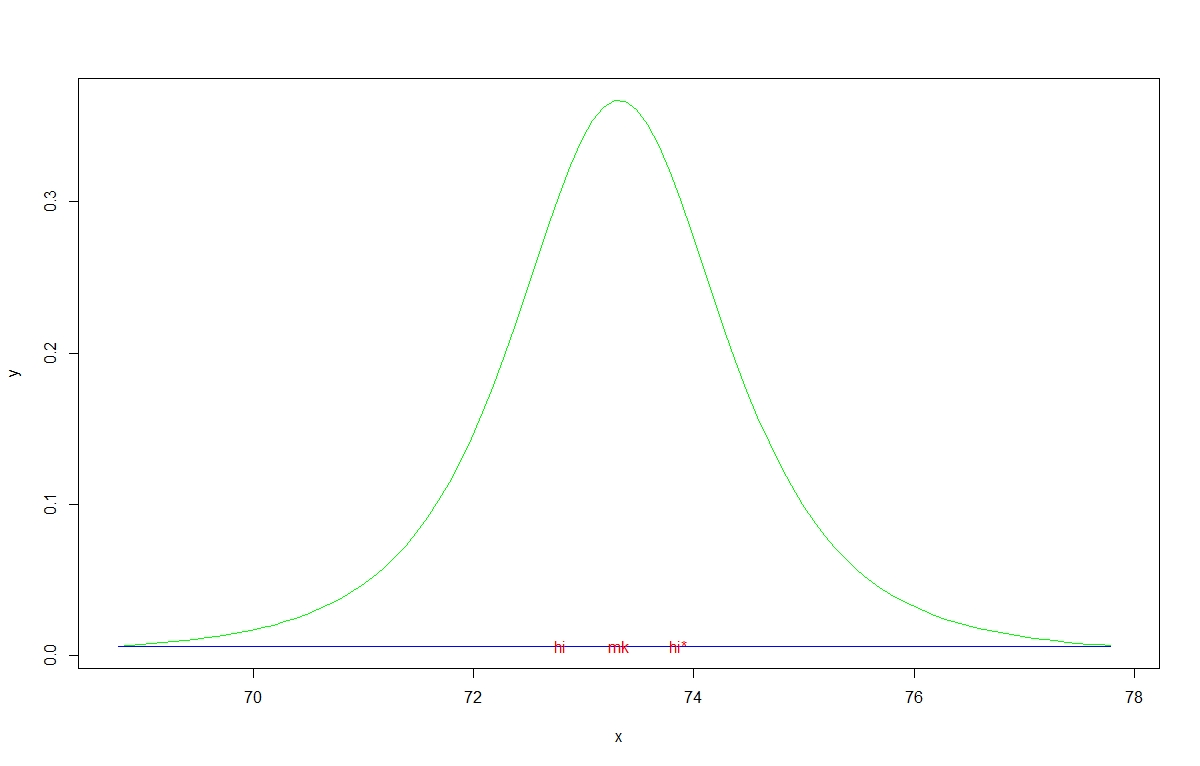
\includegraphics[width=\linewidth]{assets/distribucion-limpia-student.jpeg}
		\caption{T-Student}
		\label{fig:subim1}
	\end{subfigure}
	\begin{subfigure}{0.5\textwidth}
		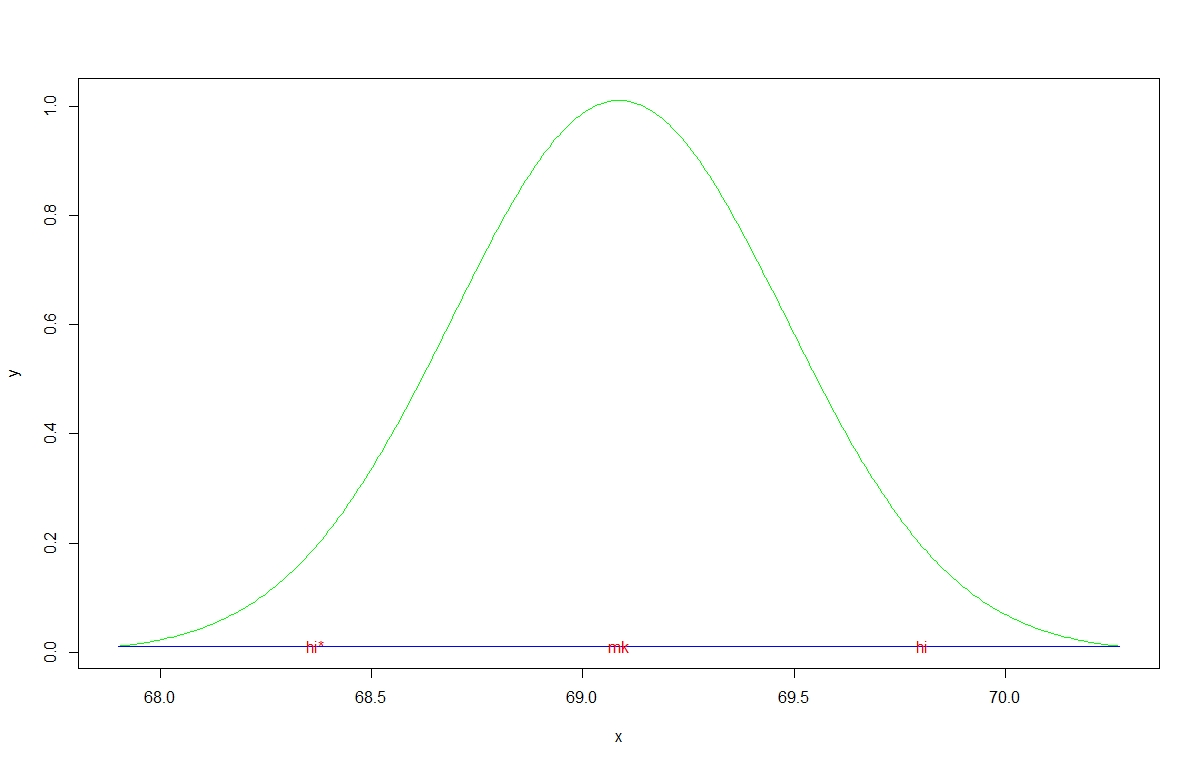
\includegraphics[width=\linewidth]{assets/distribucion-limpia-normal.jpeg}
		\caption{Gaussiana}
		\label{fig:subim2}
	\end{subfigure}
	\caption{Distribuciones vacías}
	\label{fig:image1}
\end{figure}

Lo siguiente que hay que hacer es dibujar el área de p-valor, para ello se realiza el dibujo en dos partes, primero un lado del dibujo y luego el otro lado. Para ello se utiliza la función \textit{rellenar\_area} que dibuja desde un valor hacia arriba o hacia abajo dependiendo de los valores que se le pase y de la distribución que se le utilice.

\inputminted[firstline=55, lastline=85]{R}{../R/dependencias.R}

Esto requiere pasar los valores correctos a la función, con lo que necesitamos modificar un poco el llamamiento a la función, hay que llamarla dos veces y hay que llamarla de manera correcta:

\inputminted[autogobble, firstline=48, lastline=54]{R}{../R/media.R}

Finalmente se añade un título que identifique al gráfico con la función \textit{escribir\_titulo}:

\inputminted[firstline=49, lastline=52]{R}{../R/dependencias.R}

Y así resultan los gráficos una vez aplicadas las funciones \textit{rellenar\_area} y \textit{escribir\_titulo}:

\begin{figure}[h]
	\begin{subfigure}{0.5\textwidth}
		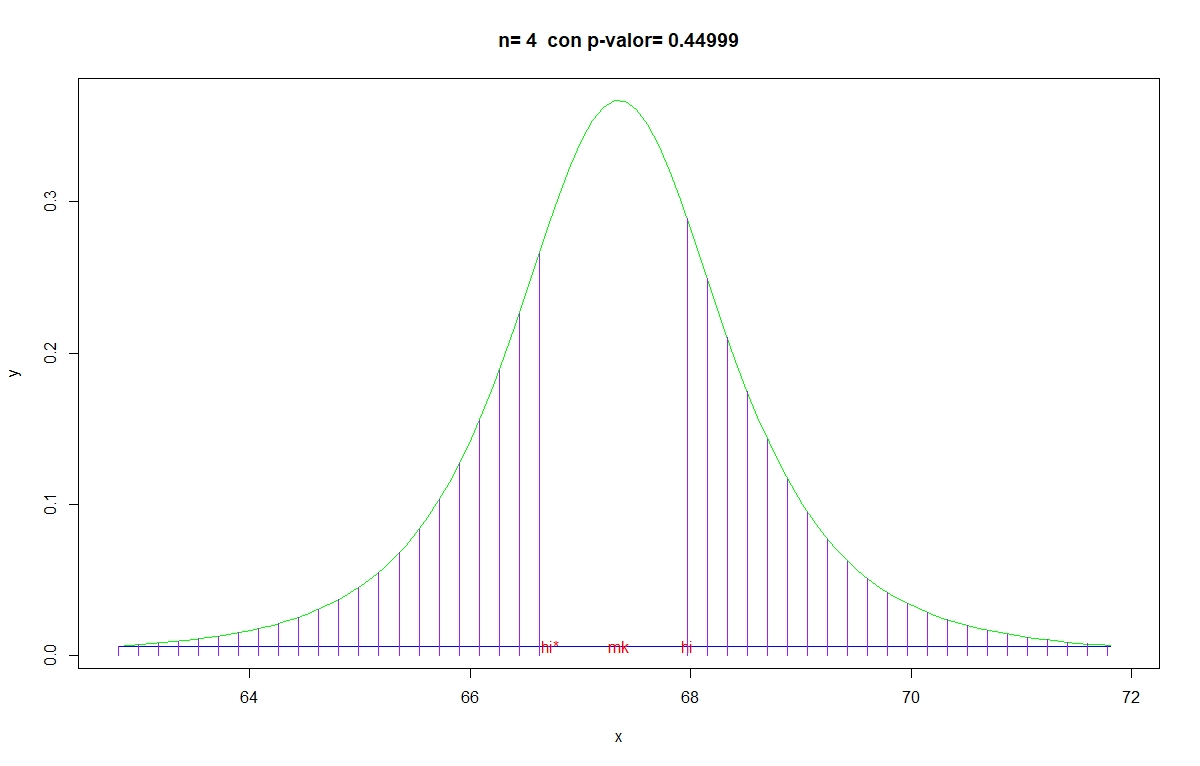
\includegraphics[width=\linewidth]{assets/grafico-completo-student.jpeg}
		\caption{T-Student}
		\label{fig:subim3}
	\end{subfigure}
	\begin{subfigure}{0.5\textwidth}
		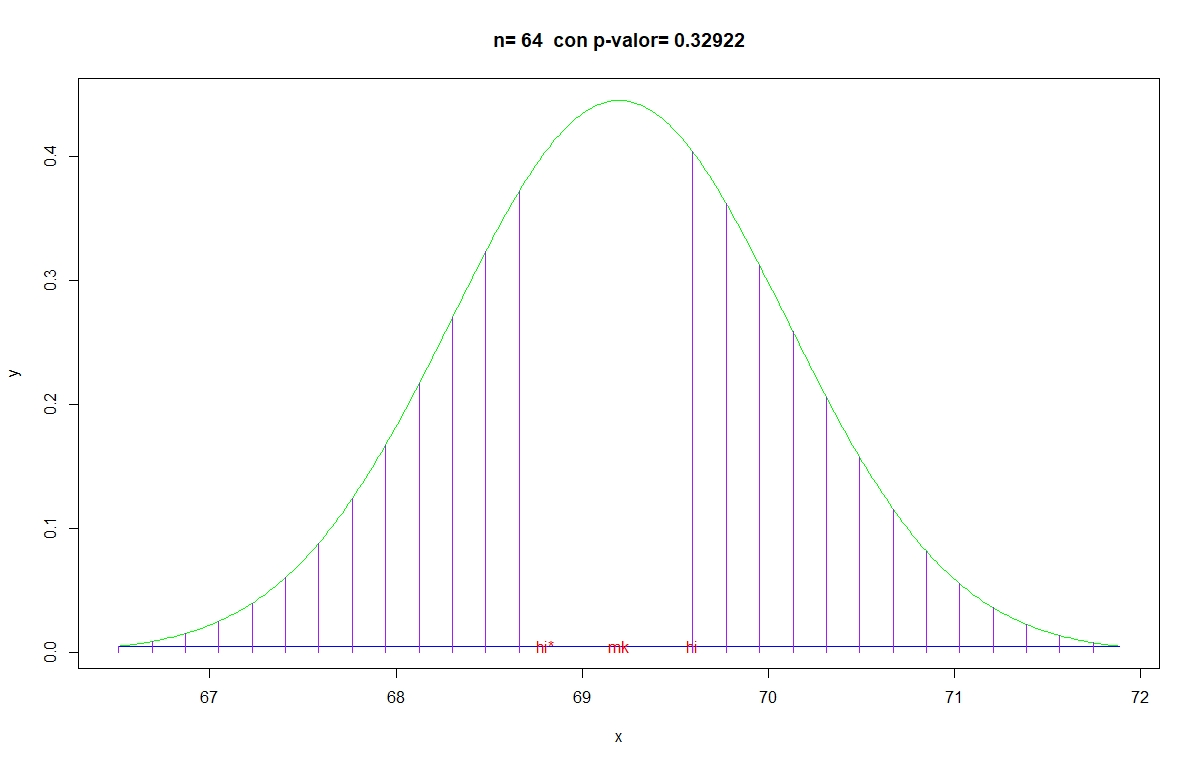
\includegraphics[width=\linewidth]{assets/grafico-completo-normal.jpeg}
		\caption{Gaussiana}
		\label{fig:subim4}
	\end{subfigure}
	\caption{Distribuciones rellenadas}
	\label{fig:image2}
\end{figure}

Una vez dibujado y calculado todo solo queda rechazar o aceptar la hipótesis, para ello se utilizan las siguientes condiciones:

\begin{itemize}
	\item Si $p-valor > 0.01$ se acepta la hipótesis y se termina el proceso.
	\item Si $0.001 < p-valor < 0.01$, se mantiene al hipótesis y se aumenta el tamaño de la muestra.
	\item Si $p-valor < 0.001$, se rechaza la hipótesis, se actualiza la media muestral actual y se aumenta el tamaño de la muestra.
\end{itemize}

Esto se traduce en el siguiente código:

\inputminted[firstline=101]{R}{../R/dependencias.R}
